\documentclass{article}
\usepackage[landscape]{geometry}
\usepackage[utf8]{inputenc}
\usepackage{tikz}
\usetikzlibrary{mindmap,backgrounds}
\pagestyle{empty}
\usepackage[T1]{fontenc}
\usepackage[utf8]{inputenc}
%lmodern	lmss
\usepackage{helvet}

\begin{document}
\pagestyle{empty}


{\fontfamily{hvt}
\centering
\begin{figure}
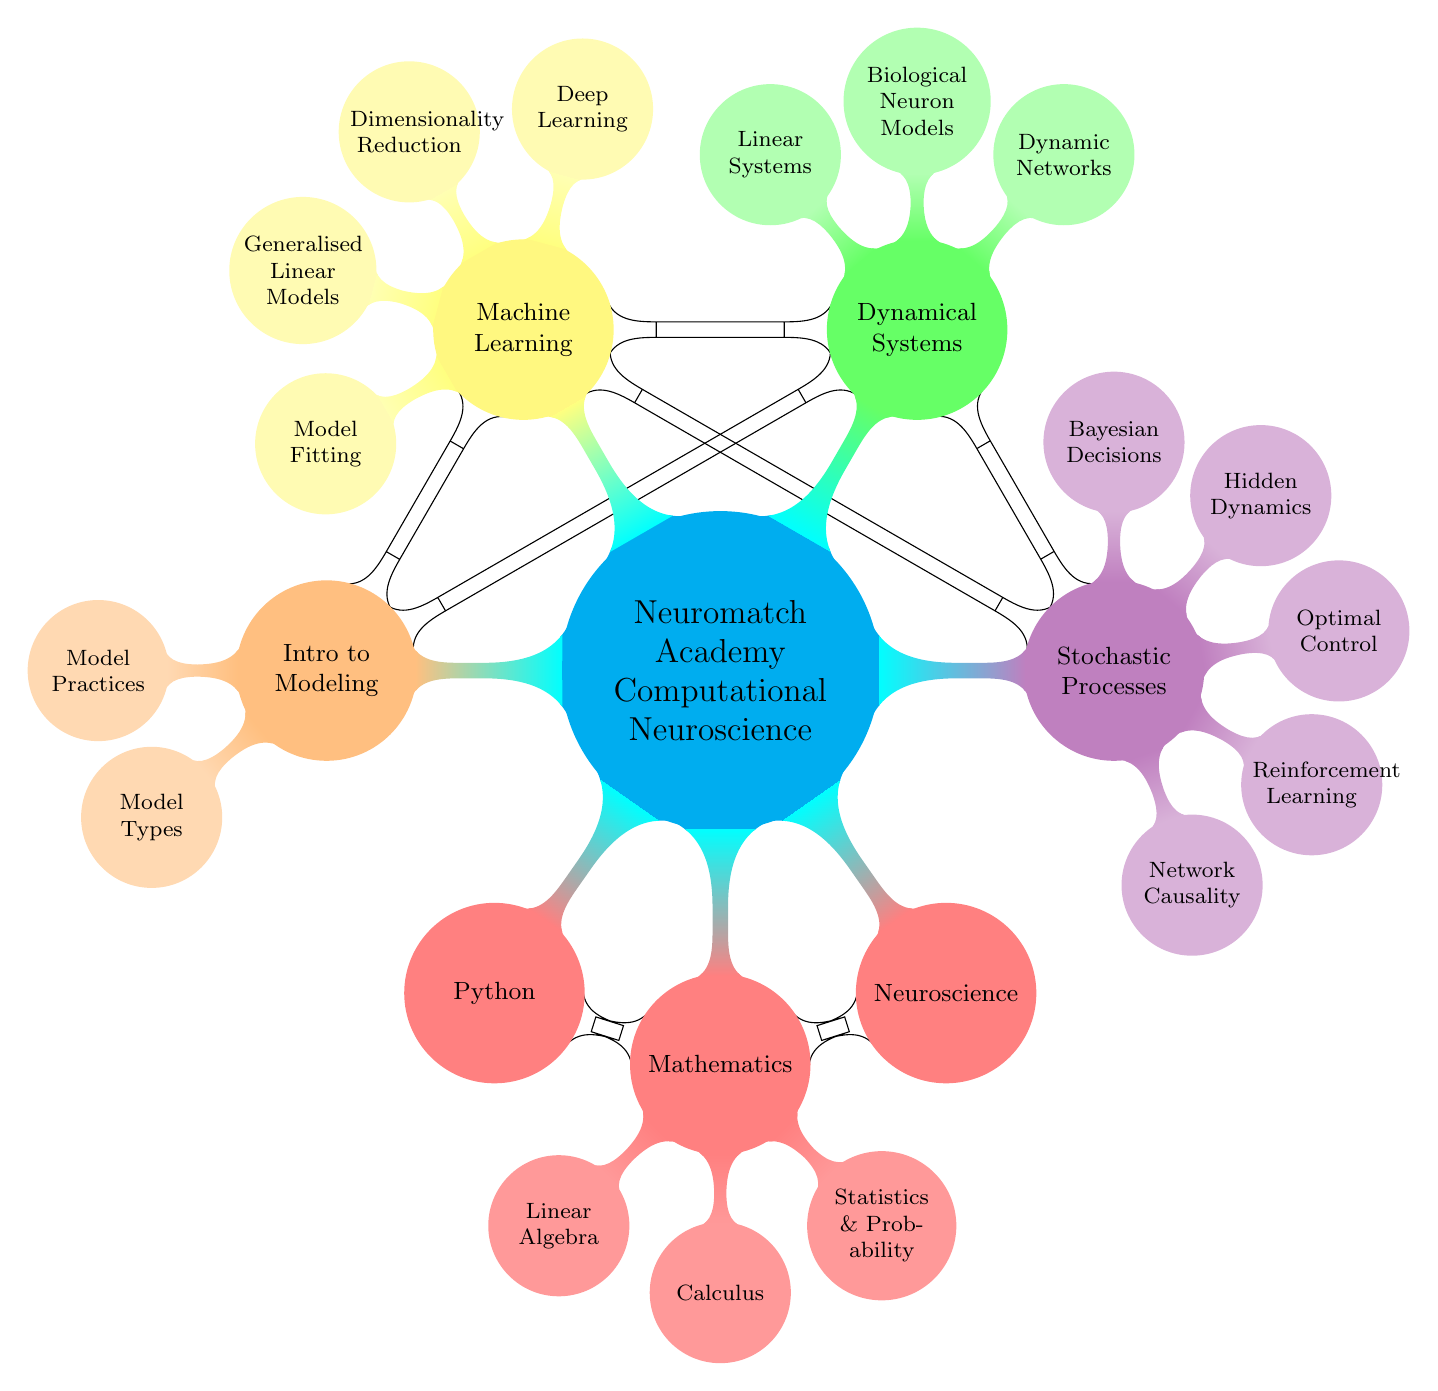
\begin{tikzpicture}




  
  \path[mindmap,concept color=cyan,text=black]
    node[concept,concept color=cyan!100](pde) {Neuromatch Academy \\ Computational Neuroscience} 
    child[grow=235,concept color=red!50] { node[concept](Pyth) {Python} 
    }   
    child[grow=305,concept color=red!50] { node[concept](Neuro) {Neuroscience} 
    }
    child[grow=270,concept color=red!50]{node[concept] (Math){ Mathematics}    
    child[grow=225, concept color=red!40] {
      node[concept](LinAl) {Linear Algebra}
    }
    child[grow=270,concept color=red!40] { node[concept](Cal) {Calculus} }
    child[grow=315,concept color=red!40] { node[concept](Stats) {Statistics \& Probability} 
    }
    }
    % Intro to Modeling
         child[grow=180,concept color=orange!50]{node[concept] (InMod){ Intro to Modeling}
      % ModTy
      child[grow=180,concept color=orange!30]{node[concept] (ModPrac){Model Practices}    }
      child[grow=220,concept color=orange!30]{node[concept] (ModTy){Model Types}}
    }
        % Machine Learning
             child[grow=120,concept color=yellow!50]{node[concept] (MachLearn){ Machine Learning}
      % ModTy
      child[grow=210,concept color=yellow!30]{node[concept] (ModFit){Model Fitting}    }
      child[grow=165,concept color=yellow!30]{node[concept] (GenLin){Generalised Linear Models}}
      child[grow=120,concept color=yellow!30]{node[concept] (DimRed){Dimensionality Reduction }}
      child[grow=75,concept color=yellow!30]{node[concept] (DeepLearn){Deep Learning}}
    }
    % DYS SYS
       child[grow=60,concept color=green!60]{node[concept] (DySys){Dynamical  Systems}
   child [grow=130,concept color=green!30]
    {node [concept] (LinSys) {Linear Systems}
    }
    child [grow=90,concept color=green!30]
    {node [concept] (BioNeur) {Biological Neuron Models }
    }
       child [grow=50,concept color=green!30]
    {node [concept] (DynNet) {Dynamic Networks}
    }
   }
     % STOCHASTIC PROCESSES
     child[grow=0,concept color=violet!50]{node[concept] (StoPro){ Stochastic Processes}
   child[grow=90,concept color=violet!30]{node[concept] (BayDec){Bayesian Decisions }    }
      % Random Number
 child[grow=50,concept color=violet!30]{node[concept] (HidDyn){Hidden Dynamics}
   }
   child[grow=10,concept color=violet!30]{node[concept] (OptCon){Optimal Control}
   }
    child[grow=-30,concept color=violet!30]{node[concept] (ReLearn){Reinforcement Learning}
   }
       child[grow=-70,concept color=violet!30]{node[concept] (NetCau){Network Causality }
   }
    };

   \begin{pgfonlayer}{background}
    \draw [circle connection bar]
      (InMod) edge (DySys)
      (InMod) edge (MachLearn)
      (MachLearn) edge (DySys)
      (DySys) edge (StoPro)
      (MachLearn) edge (StoPro) 
      (Pyth) edge (Math)
      (Math) edge (Neuro)
      ;
  \end{pgfonlayer}
\end{tikzpicture}

\end{figure}
}
\end{document}

